How do we know a student's answer is right? We check it against the
answer key. But what if the answer key is wrong? Then every student who
gets it ``right'' is actually wrong, and we'd never know.

That is the risk with our \textbf{judge} --- the evaluator that decides
whether a generated program is correct. It is the instrument whose
readings the whole book depends on. If the judge is wrong, every number
in this book is wrong. So we build it carefully, and then we attack it.

This is the second pillar of the apparatus, and it is in some ways the
most important. The world (Chapter 4) decides what the model is
\emph{allowed} to do. The teacher (Chapter 5) supplies the material to
learn from. But the judge is the thing that decides whether the model
\emph{got it right}. A subtle way to frame the whole book: we are not
really studying the model. We are studying the model \emph{through} the
judge. So the judge's integrity sets an upper bound on the
trustworthiness of everything that follows.

\section{Why an execution-based
judge}\label{why-an-execution-based-judge}

The naive way to judge a generated program is to compare it, as text, to
the expected answer. This is cheap, and it is almost worthless. Two
programs that solve the same task can look completely different as
strings --- one uses a loop, another uses \texttt{sum()}, yet both are
correct. And two programs that look nearly identical can behave
differently. String comparison measures \emph{how the code is written},
not \emph{whether it works}. That is not what we care about.

So the judge does the thing that makes this whole task special: it
\textbf{runs} the program. It executes the generated code against hidden
tests and compares the actual \emph{output} to the expected output. This
is what gives us objective, unambiguous judgment. There is no opinion
about whether the code is elegant or the ``right'' style --- either it
returns the correct result for every test, or it does not.

\section{The four-stage pipeline}\label{the-four-stage-pipeline}

\begin{figure}
\centering
\pandocbounded{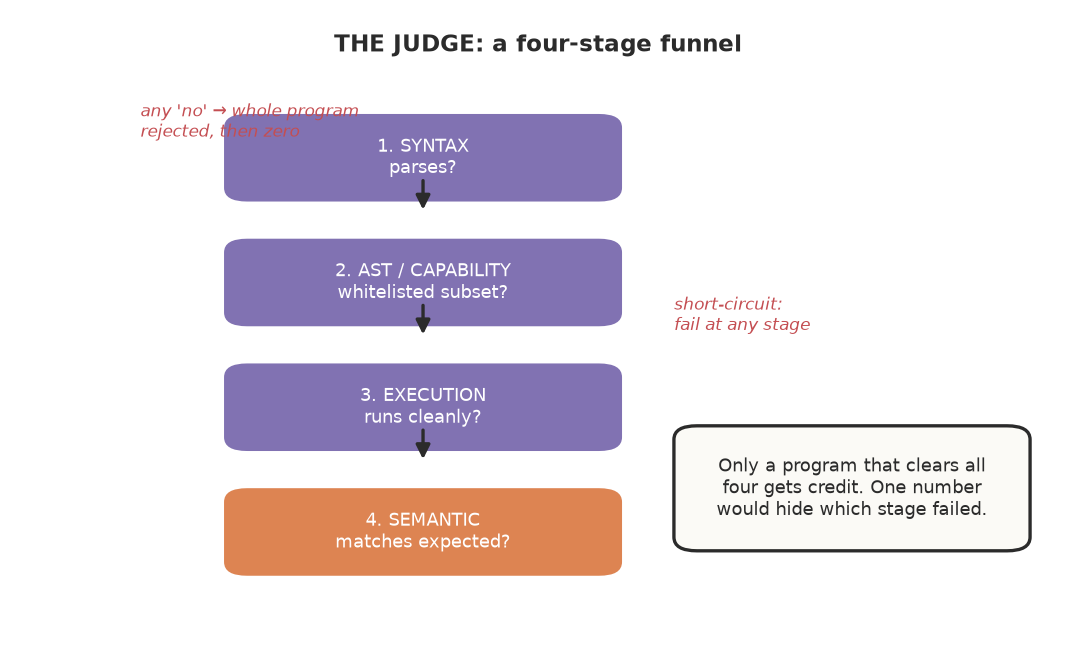
\includegraphics[keepaspectratio,alt={The judge},width=\maxwidth{\textwidth},keepaspectratio]{figures/fig_judge.png}}
\caption{The judge}
\end{figure}

The judge is a funnel: a program clears it only by passing every stage,
and the first failure sends it to zero.

We score a candidate program through four stages; a later stage only
matters if the earlier ones pass. Each stage is a filter, and each
exists for a specific reason.

\begin{enumerate}
\def\labelenumi{\arabic{enumi}.}
\tightlist
\item
  \textbf{Syntax pass} --- does the program parse as valid Python?
\item
  \textbf{AST / capability pass} --- is every node within the
  whitelisted subset? If the program smuggles in an \texttt{import}, it
  is rejected here.
\item
  \textbf{Execution pass} --- does it compile and run without error
  under the restricted environment?
\item
  \textbf{Semantic pass} --- for each hidden test, does the program's
  output match the expected output?
\end{enumerate}

The primary metric is \textbf{problem-level hidden-test pass@1}: did the
one program produced pass \emph{every} hidden test for that problem?

Why four stages rather than one? Because each stage isolates a
\emph{different} kind of failure, and separating them tells us
\emph{why} a program failed. A syntax error is a very different problem
from a capability violation (the model tried to use something outside
its world), which is different again from a runtime error (the code ran
but crashed on a test), which is finally different from a semantic error
(the code ran but produced the wrong answer). If we collapsed all four
into one ``it failed,'' we would lose the ability to diagnose. The judge
does not just tell us right or wrong; it tells us \emph{where} things go
wrong, and that diagnostic power is worth keeping.

\section{Semantic comparison: don't trust string
equality}\label{semantic-comparison-dont-trust-string-equality}

A naive evaluator would check \texttt{output\ ==\ expected}. That fails
in subtle ways. Two programs can produce the ``same'' result that isn't
string-equal: floats with rounding, a dict with keys in a different
order, nested structures. So the judge uses a proper \textbf{semantic
comparator}:

\begin{itemize}
\tightlist
\item
  integers compared exactly,
\item
  floats compared with an explicit tolerance,
\item
  booleans compared as booleans (not as 0/1),
\item
  lists compared element-by-element, recursively,
\item
  dictionaries compared key-insensitively (order doesn't matter),
\item
  nested structures compared recursively.
\end{itemize}

The comparator itself is tested --- we don't assume it's right just
because it's simple. And the tolerance matters: floating point
arithmetic is not exact, so \texttt{0.1\ +\ 0.2} does not come out to
exactly \texttt{0.3}. A judge that demanded exact equality on floats
would reject correct programs. A judge with no tolerance at all would be
as broken as one that accepted anything. Choosing the right tolerance is
a real design decision, and it is the kind of thing that quietly shapes
every number the judge produces.

\section{Mutation testing: red-teaming the
judge}\label{mutation-testing-red-teaming-the-judge}

The most important step is treating the judge as something that must be
\emph{proven} sound. We \textbf{mutate} the reference solution into
deliberately-broken versions and ask: \emph{does the judge catch them?}

We generate mutants such as: \texttt{+} → \texttt{-},
\texttt{\textgreater{}} → \texttt{\textgreater{}=}, remove the
\texttt{return}, swap the arguments, off-by-one a loop boundary, use the
wrong variable. Then we run each mutant through the hidden tests. A good
test suite \textbf{rejects} an obviously-wrong mutant. A weak test suite
lets it pass.

The mutation score --- the fraction of wrong mutants the tests catch ---
is a measure of how much we can trust the judge. If an obviously-broken
program passes our tests, the tests are too weak, and we add more until
they discriminate.

This is the ``test the tester'' principle, and it is the reason we do
not trust the judge just because we wrote it. The judge is the
instrument of measurement, so we deliberately give it wrong inputs and
check that it rejects them. It is a rare and valuable discipline: most
people build a measuring stick and assume it measures. We deliberately
try to break ours.

\section{We caught our own judge being
wrong}\label{we-caught-our-own-judge-being-wrong}

Here is what makes this chapter honest rather than aspirational: the
very first time we evaluated our model, it \textbf{scored 0.000} ---
reported a total syntax failure on every problem. And the model wasn't
wrong. The \emph{judge} was.

The root cause was a generation bug on our side: the model produced a
complete, correct program, but it was followed by padding (null bytes),
and \texttt{ast.parse} rejects null bytes. So the judge scored a
perfectly valid program as a syntax failure. Once we truncated the
padding, the model's true score emerged: \textbf{0.897}.

That moment is worth more than any passing test. It is the book's core
lesson applied to ourselves: \textbf{never trust a number from a system
we have not audited.} If we had taken the first 0.000 at face value,
we'd have concluded the approach failed. Instead, finding the judge's
bug told us the truth --- the model was actually working.

What is striking is that this bug was not exotic. It was a small,
mundane detail --- a sentinel byte used to mark the end of a generated
program --- colliding with Python's parser. We would never have found it
by reasoning about the model. We found it because we looked at the
judge's \emph{intermediate} output (the syntax scores) rather than
jumping to the headline number, and because we already had the habit of
doubting the measurement. That habit, more than any single fix, is what
kept the book honest.

\section{The honest summary}\label{the-honest-summary}

The judge is not a helper; it is the instrument whose readings we stake
the book on. So we built it strictly (four stages, semantic comparison,
tested comparator), then we red-teamed it (mutation testing), and then
--- when it gave a suspicious answer --- we attacked it until we found
our own bug. Only a judge that survives that scrutiny deserves to be
trusted.

And the deeper lesson is one we will keep relearning: in any
measurement, the instrument is part of the experiment. The model and the
judge are both subjects. We spend almost as much effort verifying the
judge as we do training the model --- and that is not waste. That is the
only way to trust the numbers at all.
